\section{改变分布}
\label{sec:vr-change-distribution}

尾概率$\mathbb{P}(X>4)$难算，是因为按$P$抽样时样本几乎从不进入尾部。一个自然的想法是换一个更常落进尾部的分布来抽样。这样抽到的样本不再服从$P$，直接求平均会高估尾概率；但每个样本被“多抽”了多少是已知的，可以按比例把它的贡献折回去。

用质量的语言说：$P$把单位质量按密度$p$摊在样本空间上，新分布把同样的单位质量按密度$q$重新摊开。一个按$q$抽到的样本点$x$，代表它附近$q$那么多的质量；要让它替$P$说话，就要给它乘上$p(x)/q(x)$。$q$比$p$大的地方样本来得勤，每个样本分量轻；$q$比$p$小的地方样本来得少，每个样本分量重。这种做法称为\term{重要性采样}（importance sampling）。本节先验证折算的公式，再研究怎样选择新分布，最后处理目标密度只知道到一个常数倍的情形。

\subsection{换测度与权重}
\label{sec:vr-change-of-measure}

设样本空间$\mathcal{X}$上有参考测度$\mu$：$\mathcal{X}=\mathbb{R}^{d}$时取Lebesgue测度，$\mathcal{X}$可数时取计数测度。目标分布$P$关于$\mu$有密度$p$，另取一个容易抽样、密度$q$可以计算的分布$Q$，称为建议分布（第~\ref{chap:sample-generation}章的拒绝采样已经用过这个名称）。

\begin{definition}[重要性采样估计]
\label{def:vr-importance-sampling}
设$\{x:f(x)p(x)\neq0\}\subseteq\{x:q(x)>0\}$（允许相差一个$\mu$零测集）。称
\begin{equation}
 w(x)=\begin{cases}p(x)/q(x), & q(x)>0,\\ 0, & q(x)=0\end{cases}
 \label{eq:vr-importance-weight}
\end{equation}
为\term{重要性权重}（importance weight）。对独立且都服从$Q$的$X_1,\dots,X_n$，称
\begin{equation}
 \hat{I}_n^{\mathrm{IS}}=\frac1n\sum_{i=1}^{n}f(X_i)\,w(X_i)
 \label{eq:vr-is-estimator}
\end{equation}
为$I$的重要性采样估计。
\end{definition}

定义中的包含关系称为覆盖条件：凡是$fp$不为零、对积分有贡献的地方，建议分布都必须有正密度。$q=0$处的权重取值无关紧要，因为按$Q$抽样几乎不会落到那里。

\begin{theorem}[换测度恒等式]
\label{thm:vr-change-of-measure}
设覆盖条件成立且$\mathbb{E}_P[\lvert f(X)\rvert]<\infty$。则$f w$在$Q$下可积，
\begin{equation}
 \mathbb{E}_Q[f(X)w(X)]=\mathbb{E}_P[f(X)]=I ,
 \label{eq:vr-change-of-measure}
\end{equation}
所以$\hat{I}_n^{\mathrm{IS}}$无偏，并且当$n\to\infty$时$\hat{I}_n^{\mathrm{IS}}\xrightarrow{\mathrm{a.s.}}I$。若进一步有
\begin{equation}
 M(q)=\mathbb{E}_Q\bigl[f(X)^2w(X)^2\bigr]=\int_{\{q>0\}}\frac{f^2p^2}{q}\,\mathrm{d}\mu<\infty ,
 \label{eq:vr-is-second-moment}
\end{equation}
则
\begin{equation}
 \operatorname{Var}\bigl(\hat{I}_n^{\mathrm{IS}}\bigr)=\frac{M(q)-I^2}{n} .
 \label{eq:vr-is-variance}
\end{equation}
\end{theorem}

\begin{proof}
记$S=\{q>0\}$。在$S$上$w\,q=p$，所以
\[
 \mathbb{E}_Q\bigl[\lvert f w\rvert\bigr]=\int_S\lvert f\rvert\frac{p}{q}\,q\,\mathrm{d}\mu=\int_S\lvert f\rvert p\,\mathrm{d}\mu .
\]
由覆盖条件，$S$之外$\lvert f\rvert p$几乎处处为零，右边等于$\mathbb{E}_P[\lvert f\rvert]<\infty$。去掉绝对值重复同样的计算，得到式~\eqref{eq:vr-change-of-measure}。

于是$f(X_i)w(X_i)$是独立同分布、期望为$I$的可积变量。对它们的平均取期望得到无偏性；由第~\ref{chap:laws-of-large-numbers}章的强大数律得到几乎必然收敛。二阶矩有限时，单项方差为$M(q)-I^2$，独立平均的方差除以$n$。
\end{proof}

在$S$上，$w$正是$P$相对于$Q$的密度，式~\eqref{eq:vr-change-of-measure}就是\BookChapterRef{chap:measure-densities}{卷四第8章“测度的密度”}中换测度公式的一个特例。定理的两部分条件不同：无偏和一致只需要原积分绝对收敛；方差有限需要式~\eqref{eq:vr-is-second-moment}，这是加权变量在$Q$下的二阶矩，与$f$在$P$下的二阶矩不是一回事。

\paragraph{手算一遍}
用导言的尾概率演示。目标$p(x)=\mathrm{e}^{-x}$（$x>0$），$f=\mathbf{1}_{\{x>4\}}$。取建议分布$Q=\operatorname{Exp}(1/4)$，平均值为$4$，比目标常进尾部。它的密度和权重是
\[
 q(x)=\tfrac14\mathrm{e}^{-x/4},\qquad w(x)=\frac{\mathrm{e}^{-x}}{\tfrac14\mathrm{e}^{-x/4}}=4\mathrm{e}^{-3x/4} .
\]
下面用五个均匀随机数逐步演示：
\[
 u=0.37,\quad 0.81,\quad 0.06,\quad 0.52,\quad 0.23 .
\]
按第~\ref{chap:sample-generation}章的逆分位数方法，$x=-4\ln u$服从$\operatorname{Exp}(1/4)$，得到
\[
 x_1=3.977,\quad x_2=0.843,\quad x_3=11.254,\quad x_4=2.616,\quad x_5=5.879 .
\]
只有$x_3$和$x_5$超过$4$，它们的权重分别是
\[
 w(x_3)=4\mathrm{e}^{-8.440}=0.00086,\qquad w(x_5)=4\mathrm{e}^{-4.409}=0.04867 .
\]
其余三项$f=0$。于是
\[
 \hat{I}_5^{\mathrm{IS}}=\frac{0.00086+0.04867}{5}=0.00991 .
\]
真值是$0.01832$。五个样本的估计当然粗糙，但它不是零。用同样五个$u$按$x=-\ln u$生成$\operatorname{Exp}(1)$样本，得到的五个值都小于$3$，直接平均给出$0$。

\begin{BookInlineFigure}
 \centering
 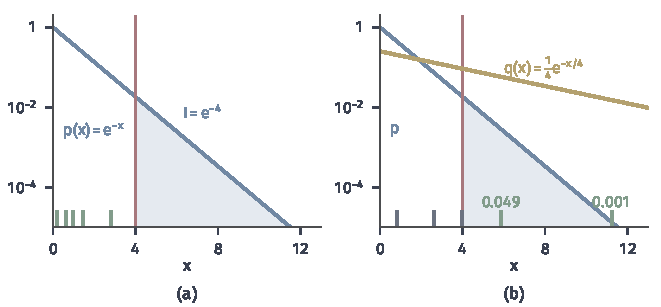
\includegraphics[width=112mm]{figures/07-probability/08-sampling-and-integration/matplotlib/vr-is-tail/figure.pdf}
 \caption{尾概率$I=\mathbb{P}(X>4)$的两种抽样，纵轴为对数刻度。蓝线为目标密度$p(x)=\mathrm{e}^{-x}$，浅蓝区域是$x>4$的尾部，红线是阈值。(a)用$u=0.37,0.81,0.06,0.52,0.23$按$x=-\ln u$生成的五个样本（绿色短线），全部落在阈值左侧。(b)同一组$u$按$x=-4\ln u$从黄线所示的$q$生成；越过阈值的两个样本为绿色并标出权重$w=4\mathrm{e}^{-3x/4}$，其余为灰色。}
 \label{fig:vr-is-tail}
\end{BookInlineFigure}

图~\ref{fig:vr-is-tail}对比了两种抽样。要算这一估计的方差，按式~\eqref{eq:vr-is-second-moment}在尾部积分：
\[
 M(q)=\int_4^{\infty}\frac{\mathrm{e}^{-2x}}{\tfrac14\mathrm{e}^{-x/4}}\,\mathrm{d}x=4\int_4^{\infty}\mathrm{e}^{-7x/4}\,\mathrm{d}x=\frac{16}{7}\mathrm{e}^{-7}\approx0.002084 .
\]
减去$I^2\approx0.000335$，单样本方差约为$0.001749$，只有直接平均的$0.01798$的$1/10.3$。这正是第~\ref{sec:vr-comparison}节例子中用到的数值。

\paragraph{覆盖条件去掉会怎样}
若建议分布只在$(0,6)$上有正密度，例如把$\operatorname{Exp}(1/4)$截断在$6$以内，$x>6$这部分尾部永远抽不到。重复定理的证明，估计的期望变为
\[
 \int_{\{q>0\}}f p\,\mathrm{d}\mu=\int_4^{6}\mathrm{e}^{-x}\,\mathrm{d}x=\mathrm{e}^{-4}-\mathrm{e}^{-6}\approx0.01584 ,
\]
比$I$少了$\mathrm{e}^{-6}/\mathrm{e}^{-4}\approx13.5\%$。这一偏差不随$n$减小，样本再多也只是越来越准地算出一个错误的数。

\paragraph{无偏而方差无穷}
仍对同一尾概率，改取$Q=\operatorname{Exp}(\lambda)$。对一般的$\lambda>0$，
\[
 M(q)=\int_4^{\infty}\frac{\mathrm{e}^{-2x}}{\lambda\mathrm{e}^{-\lambda x}}\,\mathrm{d}x=\frac1\lambda\int_4^{\infty}\mathrm{e}^{-(2-\lambda)x}\,\mathrm{d}x .
\]
$\lambda<2$时积分有限；$\lambda\geq2$时被积函数不衰减，$M(q)=\infty$。覆盖条件对每个$\lambda$都成立，所以估计都无偏、都收敛；但$\lambda\geq2$时方差为无穷。

$\lambda=2.5$时问题看得很清楚。建议样本进入尾部的概率只有$\mathrm{e}^{-10}\approx4.5\times10^{-5}$，而一旦进入，权重$w=0.4\mathrm{e}^{1.5x}$至少是$0.4\mathrm{e}^{6}\approx161$。估计值大部分时间是零，偶尔被一个巨大的权重拉高。图~\ref{fig:vr-is-running-mean}比较了两种$\lambda$下的运行平均：$\lambda=1/4$的三条路径平稳地收拢到真值；$\lambda=2.5$的三条路径在$n=2\times10^{5}$时分别只有$8$、$9$、$16$个尾部样本，终值为真值的$0.85$、$0.67$、$1.41$倍，路径呈台阶状跳动。

\begin{BookInlineFigure}
 \centering
 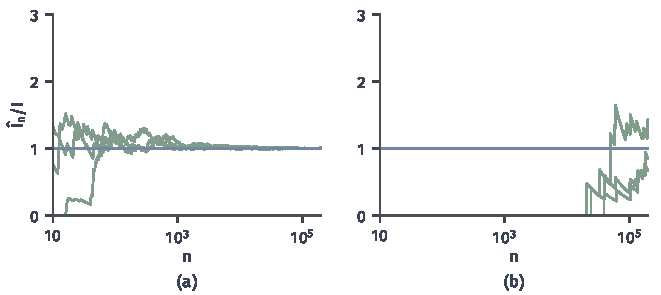
\includegraphics[width=112mm]{figures/07-probability/08-sampling-and-integration/matplotlib/vr-is-running-mean/figure.pdf}
 \caption{重要性采样估计的运行平均除以真值$I=\mathrm{e}^{-4}$，横轴为样本数（对数刻度），每图三条路径（种子11、12、13）。(a)$Q=\operatorname{Exp}(1/4)$，加权变量方差有限；(b)$Q=\operatorname{Exp}(2.5)$，估计仍无偏但加权变量的二阶矩为无穷。蓝线标出比值$1$。}
 \label{fig:vr-is-running-mean}
\end{BookInlineFigure}

\subsection{建议分布的选择}
\label{sec:vr-proposal-choice}

上一小节说明，权重公式正确只保证无偏；估计好不好，取决于式~\eqref{eq:vr-is-second-moment}的二阶矩$M(q)$。选择建议分布分两步。先从$M(q)$出发问：什么样的$q$最好？答案通常无法直接使用，于是再问：怎样用一次试运行拟合出一个可用的$q$，并且不破坏正式估计的性质？

\subsubsection{理想建议分布}
\label{sec:vr-ideal-proposal}

单样本方差是$M(q)-I^2$，其中$I$与$q$无关，所以比较建议分布就是比较$M(q)$。式~\eqref{eq:vr-is-second-moment}的被积函数是$f^2p^2/q$：分子大的地方，$q$也必须大，否则这一项会被放大。分子由$\lvert f\rvert p$决定，它衡量的是每个位置对积分的贡献，而不是样本在$P$下出现的频繁程度。

\begin{theorem}[理想建议分布]
\label{thm:vr-ideal-proposal}
设$0<\mathbb{E}_P[\lvert f(X)\rvert]<\infty$。对每个满足覆盖条件的密度$q$，
\begin{equation}
 M(q)\geq\bigl(\mathbb{E}_P[\lvert f(X)\rvert]\bigr)^2 ,
 \label{eq:vr-is-lower-bound}
\end{equation}
等号当且仅当$q$与
\begin{equation}
 q^{*}(x)=\frac{\lvert f(x)\rvert\,p(x)}{\mathbb{E}_P[\lvert f(X)\rvert]}
 \label{eq:vr-ideal-proposal}
\end{equation}
$\mu$几乎处处相等时成立。
\end{theorem}

\begin{proof}
记$S=\{q>0\}$，$a=\mathbb{E}_P[\lvert f\rvert]$。由覆盖条件，$a=\int_S\lvert f\rvert p\,\mathrm{d}\mu$。把被积函数拆成两个因子，用Cauchy--Schwarz不等式：
\[
 a=\int_S\frac{\lvert f\rvert p}{\sqrt{q}}\cdot\sqrt{q}\,\mathrm{d}\mu\leq\Bigl(\int_S\frac{f^2p^2}{q}\,\mathrm{d}\mu\Bigr)^{1/2}\Bigl(\int_S q\,\mathrm{d}\mu\Bigr)^{1/2} .
\]
右边第二个因子是$1$，第一个因子是$M(q)^{1/2}$，平方即得式~\eqref{eq:vr-is-lower-bound}。

等号成立当且仅当两个因子在$S$上几乎处处成比例，即存在常数$k$使$\lvert f\rvert p=k\,q$在$S$上几乎处处成立。两边在$S$上积分，得$k=a$，所以$q=\lvert f\rvert p/a$在$S$上几乎处处成立。在$S$之外$q=0$，而由覆盖条件$\lvert f\rvert p$也几乎处处为零。所以$q=q^{*}$几乎处处成立。反过来，$q=q^{*}$时直接计算得$M(q^{*})=a^2$。
\end{proof}

最小的单样本方差是$a^2-I^2$。$f$在$P$下几乎必然不变号时$\lvert I\rvert=a$，最小方差为零：每个样本的$f w$恰好等于$I$。$f$变号时$a>\lvert I\rvert$，即使用理想建议，方差也不为零。

\paragraph{尾概率：零方差与循环}
尾概率中$f=\mathbf{1}_{\{x>4\}}$不变号，$a=I=\mathrm{e}^{-4}$，理想建议是
\[
 q^{*}(x)=\frac{\mathrm{e}^{-x}\mathbf{1}_{\{x>4\}}}{\mathrm{e}^{-4}}=\mathrm{e}^{-(x-4)}\mathbf{1}_{\{x>4\}} ,
\]
也就是在$X>4$条件下$X$的分布。按它抽样，每个样本都落在尾部，权重是常数：
\[
 w(x)=\frac{\mathrm{e}^{-x}}{\mathrm{e}^{-(x-4)}}=\mathrm{e}^{-4},\qquad x>4 .
\]
一个样本就给出精确的$I$。问题在于$q^{*}$的归一化常数正是$a=I$：写出$q^{*}$，等于已经知道了答案。这里能写出来，只是因为指数分布的尾部恰好还是指数分布。一般地，理想建议告诉我们抽样应当往哪里集中，而不是一个可以直接使用的分布。

\paragraph{变号的被积函数}
取$P=\mathcal{N}(0,1)$，$f(x)=x$，$I=0$。此时$a=\mathbb{E}\lvert X\rvert=\sqrt{2/\pi}$，理想建议
\[
 q^{*}(x)=\frac{\lvert x\rvert\varphi(x)}{\sqrt{2/\pi}}
\]
在原点处为零、在$\pm1$附近各有一个峰。它的单样本方差是
\[
 a^2-I^2=\frac{2}{\pi}\approx0.637 ,
\]
比直接平均的$\operatorname{Var}(X)=1$小，但不为零：正负两部分的样本各自带着符号，平均时仍有波动。若把$f$拆成正部$f^{+}=\max\{f,0\}$与负部$f^{-}=\max\{-f,0\}$，分别用各自的理想建议计算再相减，两部分都是零方差。图~\ref{fig:vr-ideal-proposal}画出两个例子中的$p$、贡献$\lvert f\rvert p$与$q^{*}$。

\begin{BookInlineFigure}
 \centering
 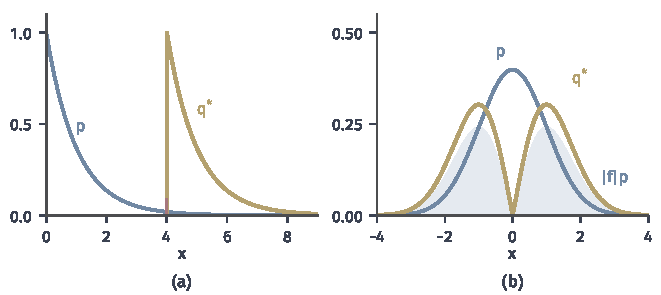
\includegraphics[width=112mm]{figures/07-probability/08-sampling-and-integration/matplotlib/vr-ideal-proposal/figure.pdf}
 \caption{理想建议分布$q^{*}=\lvert f\rvert p/\mathbb{E}_P\lvert f\rvert$（黄线）与目标密度$p$（蓝线）。(a)$p(x)=\mathrm{e}^{-x}$，$f=\mathbf{1}_{\{x>4\}}$：$q^{*}$是平移到$4$的指数密度，贡献$\lvert f\rvert p$为$x>4$下方面积$\mathrm{e}^{-4}$，在此刻度下几乎看不见。(b)$p=\mathcal{N}(0,1)$，$f(x)=x$：浅蓝区域为$\lvert x\rvert\varphi(x)$，$q^{*}$是它除以$\sqrt{2/\pi}$，在原点为零。}
 \label{fig:vr-ideal-proposal}
\end{BookInlineFigure}

\paragraph{在分布族内选择}
既然$q^{*}$通常不可用，退一步在一个可采样的族中找使$M(q)$最小的成员。尾概率中取$Q=\operatorname{Exp}(\lambda)$，上一小节已经算出，$0<\lambda<2$时
\begin{equation}
 v(\lambda)=M(q_\lambda)-I^2=\frac{\mathrm{e}^{-4(2-\lambda)}}{\lambda(2-\lambda)}-\mathrm{e}^{-8} .
 \label{eq:vr-exp-family-variance}
\end{equation}
对第一项取对数，得到$4\lambda-8-\ln\lambda-\ln(2-\lambda)$，令它的导数为零：
\[
 4-\frac1\lambda+\frac{1}{2-\lambda}=0 .
\]
两边乘$\lambda(2-\lambda)$整理，得
\[
 4\lambda^2-10\lambda+2=0 .
\]
在$(0,2)$内的根是$\lambda^{*}=(5-\sqrt{17})/4\approx0.219$，此时$v(\lambda^{*})\approx0.001730$，比直接平均小$10.4$倍。$\lambda^{*}$对应的平均值$1/\lambda^{*}\approx4.56$略大于阈值$4$：抽样集中在尾部的起点附近，那里正是$\lvert f\rvert p$最大的地方。

\begin{BookInlineFigure}
 \centering
 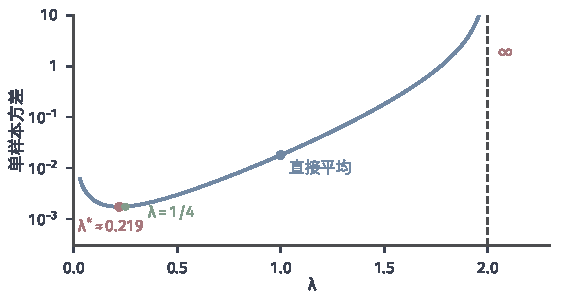
\includegraphics[width=96mm]{figures/07-probability/08-sampling-and-integration/matplotlib/vr-is-second-moment/figure.pdf}
 \caption{尾概率$\mathbb{P}(X>4)$用$Q=\operatorname{Exp}(\lambda)$作建议时的单样本方差$v(\lambda)$，纵轴为对数刻度。蓝点$\lambda=1$即直接平均，红点为最优$\lambda^{*}\approx0.219$，绿点为正文例子用的$\lambda=1/4$；虚线$\lambda=2$右侧方差为无穷。}
 \label{fig:vr-is-second-moment}
\end{BookInlineFigure}

图~\ref{fig:vr-is-second-moment}画出$v(\lambda)$。曲线有两个陡峭的方向。$\lambda\to0$时建议分布摊得过宽，大部分样本落在远离阈值、贡献极小的地方；$\lambda\to2$时建议分布的尾部衰减得和$p^2$一样快，权重平方在远处不再衰减，二阶矩发散。后一种情形是更危险的一侧：它不表现为估计变差一点，而是方差直接变为无穷。

\paragraph{尾部过轻}
这个现象有一般的形式。$f$有界时，$M(q)\leq\sup\lvert f\rvert^2\,\mathbb{E}_P[w]$，若$q$的尾部至少和$p$一样重，使$w=p/q$有界，则$M(q)$有限。反之，若在某个方向上$q$比$p$衰减得快很多，$w$在那里无界，$f^2p^2/q$可能不可积。所以选建议分布时，宁可尾部偏重，不可偏轻。

\subsubsection{试运行中的拟合}
\label{sec:vr-pilot-fitting}

当理想建议无法直接写出时，可以先用一个覆盖面足够宽的分布$q_0$做一次试运行，从试运行样本中看出贡献集中在哪里，再从一个可采样、密度可计算的族中挑出与$q^{*}$相近的成员。

\paragraph{主要思想}
设$Y_1,\dots,Y_m$独立且都服从$q_0$，$q_0$覆盖$fp$。记
\begin{equation}
 c_j=\frac{\lvert f(Y_j)\rvert\,p(Y_j)}{q_0(Y_j)},\qquad j=1,\dots,m .
 \label{eq:vr-pilot-contribution}
\end{equation}
由换测度恒等式，对任意使积分存在的函数$g$，
\[
 \mathbb{E}_{q_0}\bigl[c\,g(Y)\bigr]=\int\lvert f\rvert p\,g\,\mathrm{d}\mu=a\,\mathbb{E}_{q^{*}}[g] .
\]
所以以$c_j$为权重的加权平均$\sum_j c_jg(Y_j)/\sum_j c_j$近似$\mathbb{E}_{q^{*}}[g]$：带权重$c_j$的试运行样本是$q^{*}$的一个粗略画像，$c_j$可以看成第$j$个试运行点对积分的贡献。

拟合时在族中挑出各项矩与这个画像一致的成员。以方差为$1$的正态位置族$\mathcal{N}(m,1)$为例，与$q^{*}$的KL散度为
\[
 D_{\mathrm{KL}}\bigl(q^{*}\Vert\mathcal{N}(m,1)\bigr)=\int q^{*}\ln q^{*}\,\mathrm{d}x+\frac12\ln(2\pi)+\frac12\mathbb{E}_{q^{*}}\bigl[(X-m)^2\bigr] .
\]
只有最后一项依赖$m$，它在$m=\mathbb{E}_{q^{*}}[X]$时最小。把$\mathbb{E}_{q^{*}}[X]$换成加权平均，就得到以贡献为权重的均值。用KL散度逼近一个分布的一般讨论见第~\ref{chap:distribution-approximation}章。

贡献集中在几个分离的区域时，每个区域配一个成分，成分的权重取该区域贡献所占的比例。再留一份$q_0$本身作为\term{防御性混合}（defensive mixture）成分：
\begin{equation}
 q=\alpha\,q_0+(1-\alpha)\sum_{k=1}^{K}\pi_k\,\mathcal{N}(m_k,1),\qquad 0<\alpha<1 .
 \label{eq:vr-defensive-mixture}
\end{equation}
这一份保证了$q\geq\alpha q_0$，于是$w=p/q\leq p/(\alpha q_0)$：只要$p/q_0$有界，权重就有界，拟合得再差，二阶矩也不会发散；试运行没有看到的区域，也仍以$\alpha q_0$的密度被抽到。

\paragraph{计算过程}
下面结合一个两区域的例子写出计算过程。目标$P=\mathcal{N}(0,1)$，
\[
 f(x)=\mathbf{1}_{\{x<-2.5\}}+\mathbf{1}_{\{x>3\}} ,
\]
真值$I=\Phi(-2.5)+1-\Phi(3)=0.006210+0.001350=0.007560$，左侧贡献占$82\%$。直接平均的单样本方差为$I(1-I)\approx0.007502$。

\needspace{6\baselineskip}
\paragraph{变量}
\begin{itemize}
 \item 试运行分布$q_0$与试运行样本$Y_1,\dots,Y_m$；例中$q_0=\mathcal{N}(0,3^2)$，$m=30$。
 \item 贡献$c_j$，按式~\eqref{eq:vr-pilot-contribution}计算，长度为$m$的非负数组。
 \item 区域划分及区域数$K$；例中按符号分为左右两区，$K=2$。
 \item 拟合参数：成分权重$\pi_k$与成分均值$m_k$，$k=1,\dots,K$；防御比例$\alpha$，例中$\alpha=0.2$。
\end{itemize}

\needspace{6\baselineskip}
\paragraph{步骤}
\begin{enumerate}
 \item \textbf{试运行。}抽取$Y_1,\dots,Y_m\sim q_0$，计算各$c_j$。例中（种子3）$30$个点里有$9$个落进贡献区，其中只有$4$个的贡献不可忽略：
 \[
 \begin{array}{lcccc}
  y_j & -3.165 & -2.596 & 3.007 & 4.637\\
  c_j & 0.03492 & 0.15020 & 0.05394 & 0.00021
 \end{array}
 \]
 另外$5$个点落在$\lvert y\rvert>5.8$处，那里$p$极小，贡献都小于$10^{-6}$。

 \item \textbf{按区域汇总。}对每个区域$k$计算贡献之和$s_k$。例中
 \[
  s_1=0.03492+0.15020=0.18512,\qquad s_2=0.05394+0.00021=0.05415 .
 \]

 \item \textbf{成分权重。}取$\pi_k=s_k/\sum_l s_l$。例中
 \[
  \pi_1=\frac{0.18512}{0.23927}=0.774,\qquad \pi_2=0.226 .
 \]
 真实比例是$0.821$与$0.179$，三十个试运行点给出的估计已经大致正确。

 \item \textbf{成分均值。}取$m_k=\sum_{j\in k}c_jy_j/s_k$。例中
 \[
  m_1=\frac{0.03492\times(-3.165)+0.15020\times(-2.596)}{0.18512}=-2.703 ,
 \]
 同样算得$m_2=3.013$。

 \item \textbf{组装建议。}代入式~\eqref{eq:vr-defensive-mixture}。例中
 \[
  q=0.2\,\mathcal{N}(0,3^2)+0.8\bigl[0.774\,\mathcal{N}(-2.703,1)+0.226\,\mathcal{N}(3.013,1)\bigr] .
 \]
\end{enumerate}
最终得到的$q$由数值积分算得单样本方差$M(q)-I^2\approx1.99\times10^{-4}$，是直接平均的$1/37.7$。这里$p/q_0=3\mathrm{e}^{-4x^2/9}\leq3$，所以权重不超过$3/\alpha=15$。图~\ref{fig:vr-mixture-fit}左图是试运行点及其贡献，右图把拟合的$q$与$q^{*}$放在一起。

\begin{BookInlineFigure}
 \centering
 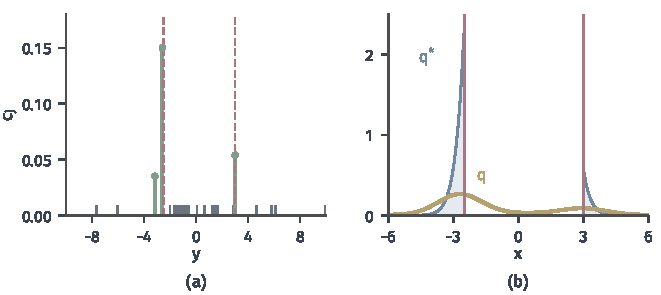
\includegraphics[width=112mm]{figures/07-probability/08-sampling-and-integration/matplotlib/vr-mixture-fit/figure.pdf}
 \caption{两区域贡献的建议拟合，$P=\mathcal{N}(0,1)$，$f=\mathbf{1}_{\{x<-2.5\}}+\mathbf{1}_{\{x>3\}}$，红色虚线或实线为两个阈值。(a)$q_0=\mathcal{N}(0,3^2)$的$30$个试运行点（种子3）：灰色短线为贡献可忽略的点，绿色竖线高度为贡献$c_j$。(b)蓝线与浅蓝区域为理想建议$q^{*}=fp/I$，黄线为拟合的防御性混合$q$。}
 \label{fig:vr-mixture-fit}
\end{BookInlineFigure}

\paragraph{没看到不等于没有}
试运行的范围不够时，拟合会漏掉区域。把试运行分布换成较窄的$q_0=\mathcal{N}(0,1.5^2)$，同样抽$30$个点（种子0），只有一个点$-3.488$落进左区，没有点越过$3$。按上面的步骤只能拟合出左侧一个成分$\mathcal{N}(-3.488,1)$。若不留防御成分，右区$x>3$只能靠这个远在左边的成分偶尔覆盖，单样本方差约为$1.3\times10^{5}$，是直接平均的$1.8\times10^{7}$倍；留下$\alpha=0.2$的$q_0$后，方差降为约$7.4\times10^{-4}$，仍比直接平均好约$10$倍。试运行中某个区域一个点也没有，只说明$m$个点没有落到那里，不说明那里对积分没有贡献。

\subsubsection{固定建议后的估计}
\label{sec:vr-fixed-proposal}

拟合出的$q$依赖试运行样本，本身是随机的。正式估计必须说明：在$q$随机的情况下，加权平均还是否无偏、方差怎样计算。

把试运行的全部结果记为$D=(Y_1,\dots,Y_m)$，拟合的建议记为$q_D$。正式计算在给定$D$后，用一组与$D$独立的新随机数抽取$X_1,\dots,X_n\sim q_D$，再计算
\[
 \hat{I}_n^{\mathrm{IS}}=\frac1n\sum_{i=1}^{n}f(X_i)\frac{p(X_i)}{q_D(X_i)} .
\]
图~\ref{fig:vr-two-stage}画出这一两阶段结构。

\begin{BookInlineFigure}
 \centering
 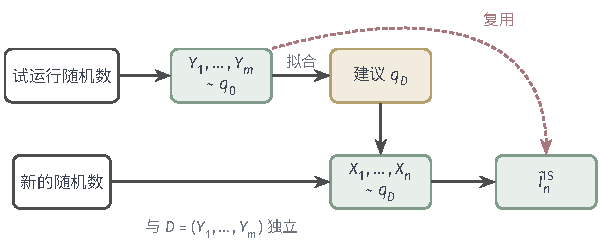
\includegraphics[width=102mm]{figures/07-probability/08-sampling-and-integration/tikz/vr-two-stage/figure.pdf}
 \caption{两阶段重要性采样。试运行随机数产生$D=(Y_1,\dots,Y_m)$并拟合建议$q_D$；正式样本由与$D$独立的新随机数按$q_D$生成。红色虚线表示把试运行点直接混入正式估计，这样做会破坏下面的条件无偏性。}
 \label{fig:vr-two-stage}
\end{BookInlineFigure}

\begin{theorem}[两阶段估计的无偏性]
\label{thm:vr-two-stage}
设$\mathbb{E}_P[\lvert f\rvert]<\infty$，对几乎每个试运行结果$D$，$q_D$都覆盖$fp$，且正式样本所用的随机数与$D$独立。则
\begin{equation}
 \mathbb{E}\bigl[\hat{I}_n^{\mathrm{IS}}\bigm|D\bigr]=I,\qquad \mathbb{E}\bigl[\hat{I}_n^{\mathrm{IS}}\bigr]=I .
 \label{eq:vr-two-stage-unbiased}
\end{equation}
若再有$\mathbb{E}[M(q_D)]<\infty$，则
\begin{equation}
 \operatorname{Var}\bigl(\hat{I}_n^{\mathrm{IS}}\bigr)=\frac{\mathbb{E}[M(q_D)]-I^2}{n} .
 \label{eq:vr-two-stage-variance}
\end{equation}
\end{theorem}

\begin{proof}
正式样本可以写成$X_i=T(D,\bm{U}_i)$，其中$\bm{U}_1,\dots,\bm{U}_n$与$D$独立，且对固定的$d$，$T(d,\bm{U}_i)$服从$q_d$。由第~\ref{chap:conditional-distributions}章，$\bm{U}_i$与$D$独立时，给定$D=d$的条件期望可以把$d$代入后只对$\bm{U}_i$求期望。对固定的$d$，这是建议$q_d$下的普通重要性采样，由定理~\ref{thm:vr-change-of-measure}，它的期望是$I$。这就是式~\eqref{eq:vr-two-stage-unbiased}的第一式；再用全期望公式得到第二式。

同样，给定$D=d$时的条件方差是$(M(q_d)-I^2)/n$。由全方差公式，总方差等于条件方差的期望加条件期望的方差；条件期望恒为$I$，后一项为零，于是得到式~\eqref{eq:vr-two-stage-variance}。
\end{proof}

定理中两个条件的作用不同。“对每个$D$都覆盖”保证无论试运行结果如何，正式估计都不偏；防御性混合使这一条自动成立，因为$q_D\geq\alpha q_0$而$q_0$覆盖$fp$。“新随机数与$D$独立”保证条件化以后正式样本确实服从$q_D$。在固定$D$下，正式样本的$f w$值独立同分布，用它们的样本方差除以$n$就可以估计条件方差。

\paragraph{复用试运行点}
如果把试运行点$Y_j$也代入同一个加权公式，即在正式平均中加入$f(Y_j)p(Y_j)/q_D(Y_j)$，问题出在两处：$Y_j$并不服从$q_D$，而是服从$q_0$；$q_D$又是由$Y_j$拟合出来的，在$Y_j$附近往往偏大。这一项的期望一般不等于$I$。试运行点可以利用，但要用它实际来源的密度：$f$非负时，$\sum_jc_j/m$就是基于$q_0$的一个无偏估计，例中为$0.00798$。正式估计在给定$D$时的条件期望恒为$I$，所以两者不相关，可以按固定的比例合并。

\paragraph{混合形式不保证有限方差}
式~\eqref{eq:vr-two-stage-variance}要求$\mathbb{E}[M(q_D)]<\infty$，这要对试运行的每种可能结果检查。混合本身不能保证这一点。仍用上面的两区域例子，如果在步骤4中同时用加权方差拟合每个成分的方差，左右两个成分的标准差分别只有$0.223$与$0.103$。没有防御成分时，$q$在远处按$\mathrm{e}^{-x^2/(2\times0.223^2)}$衰减，比$p^2\propto\mathrm{e}^{-x^2}$快得多，左区上$p^2/q$不可积，$M(q)=\infty$。加上$\alpha=0.2$的$q_0=\mathcal{N}(0,3^2)$后，权重有界，单样本方差约为$7.7\times10^{-5}$。起作用的是一个尾部足够重的成分，而不是混合这一形式。

试运行越长，拟合越可靠，但它的成本也计入总预算。试运行与正式计算之间怎样分配预算，由第~\ref{chap:sampling-budget-method-selection}章讨论。

\subsection{自归一化估计}
\label{sec:vr-self-normalized}

许多目标分布只知道到一个常数倍：能算$\widetilde{p}(x)\geq0$，而$p=\widetilde{p}/Z$中的归一化常数
\[
 Z=\int\widetilde{p}\,\mathrm{d}\mu,\qquad 0<Z<\infty
\]
无法直接计算。第~\ref{chap:sample-generation}章的拒绝采样与Metropolis--Hastings采样都只用到$\widetilde{p}$。这时权重$p/q$算不出来，只能算$\widetilde{w}=\widetilde{p}/q=Zw$。

办法是用同一批样本同时估计$Z$。由换测度恒等式，$\mathbb{E}_Q[\widetilde{w}]=Z$，$\mathbb{E}_Q[\widetilde{w}f]=ZI$，两者相除，未知的$Z$约去。

\begin{definition}[自归一化估计]
\label{def:vr-self-normalized}
设$q$覆盖整个目标，即$\{\widetilde{p}>0\}\subseteq\{q>0\}$。对独立且都服从$Q$的$X_1,\dots,X_n$，记$\widetilde{w}_i=\widetilde{p}(X_i)/q(X_i)$，称
\begin{equation}
 \hat{I}_n^{\mathrm{SN}}=\frac{\sum_{i=1}^{n}\widetilde{w}_i\,f(X_i)}{\sum_{i=1}^{n}\widetilde{w}_i}
 \label{eq:vr-self-normalized}
\end{equation}
为\term{自归一化重要性采样}（self-normalized importance sampling）估计；分母为零时规定估计值为$0$。
\end{definition}

覆盖的要求比定义~\ref{def:vr-importance-sampling}更强：分母要估计整个$Z$，所以凡是$\widetilde{p}>0$的地方都要覆盖，不能只覆盖$f\widetilde{p}\neq0$的部分。

\begin{theorem}[自归一化估计的一致性]
\label{thm:vr-sn-consistency}
设$q$覆盖整个目标且$\mathbb{E}_P[\lvert f\rvert]<\infty$。则$\hat{I}_n^{\mathrm{SN}}\xrightarrow{\mathrm{a.s.}}I$。
\end{theorem}

\begin{proof}
由换测度恒等式，$\widetilde{w}$与$\widetilde{w}f$在$Q$下可积，期望分别是$Z$与$ZI$。由强大数律，几乎必然有
\[
 \frac1n\sum_{i=1}^{n}\widetilde{w}_i\to Z,\qquad \frac1n\sum_{i=1}^{n}\widetilde{w}_if(X_i)\to ZI .
\]
因为$Z>0$，在这些样本点上分母从某个$n$起为正，比值收敛到$ZI/Z=I$。
\end{proof}

\paragraph{有限样本的偏差}
比值的期望一般不是期望的比值。最极端的情形是$n=1$：只要$\widetilde{w}_1>0$，式~\eqref{eq:vr-self-normalized}就等于$f(X_1)$，于是估计的期望是$f$在$Q$下（限制在$\widetilde{w}>0$上）的平均，而不是在$P$下的平均。另一种有限样本现象是分母为零：若$\widetilde{p}$在$q$的支撑上有一部分为零，所有样本都可能落在那里，这时估计没有信息。

用一个能手算的例子看这些量。目标$\widetilde{p}(x)=x^2\mathrm{e}^{-x}$（$x>0$），它是$\operatorname{Gamma}(3,1)$的未归一化密度，$Z=2$；要算$I=\mathbb{E}_P[X]=3$。建议$Q=\operatorname{Exp}(1/2)$，于是
\[
 q(x)=\tfrac12\mathrm{e}^{-x/2},\qquad \widetilde{w}(x)=2x^2\mathrm{e}^{-x/2} .
\]
$n=1$时估计的期望是$\mathbb{E}_Q[X]=2$，偏差为$-1$。仍用前面那五个均匀数，按$x=-2\ln u$生成五个建议样本：
\[
 x=1.989,\quad 0.421,\quad 5.627,\quad 1.308,\quad 2.939 .
\]
对应的权重为
\[
 \widetilde{w}=2.926,\quad 0.288,\quad 3.799,\quad 1.779,\quad 3.974 .
\]
权重和为$12.766$，加权和$\sum\widetilde{w}_ix_i=41.326$，于是
\[
 \hat{I}_5^{\mathrm{SN}}=\frac{41.326}{12.766}=3.237 .
\]
副产品是$Z$的无偏估计$12.766/5=2.553$。

\paragraph{渐近误差}
把误差写成
\[
 \hat{I}_n^{\mathrm{SN}}-I=\frac{\frac1n\sum_{i=1}^{n}\widetilde{w}_i\bigl(f(X_i)-I\bigr)}{\frac1n\sum_{i=1}^{n}\widetilde{w}_i} .
\]
分子是独立同分布变量$\widetilde{w}(f-I)$的平均，它的期望是$ZI-IZ=0$。若中心化加权量的二阶矩
\begin{equation}
 \tau^2=\mathbb{E}_Q\bigl[\widetilde{w}(X)^2\bigl(f(X)-I\bigr)^2\bigr]<\infty ,
 \label{eq:vr-sn-tau}
\end{equation}

由第~\ref{chap:central-limit-theorem}章的中心极限定理，分子乘以$\sqrt{n}$依分布收敛到$\mathcal{N}(0,\tau^2)$；分母几乎必然收敛到$Z$。由第~\ref{chap:weak-convergence-of-distributions}章的Slutsky定理，
\begin{equation}
 \sqrt{n}\,\bigl(\hat{I}_n^{\mathrm{SN}}-I\bigr)\xrightarrow{\mathrm{d}}\mathcal{N}\Bigl(0,\frac{\tau^2}{Z^2}\Bigr) .
 \label{eq:vr-sn-clt}
\end{equation}
要检查的是$\widetilde{w}(f-I)$的二阶矩，而不是$\widetilde{w}f$的二阶矩：减去$I$以后，大权重落在$f\approx I$处的样本不再放大误差。式~\eqref{eq:vr-sn-clt}是渐近结论，它不给出任何固定$n$下的覆盖保证。

把分母写成$Z(1+\delta)$，$\delta$是分母的相对误差，展开$1/(1+\delta)\approx1-\delta$并取期望，可以得到偏差的主项：
\begin{equation}
 \mathbb{E}\bigl[\hat{I}_n^{\mathrm{SN}}\bigr]-I\approx-\frac{\mathbb{E}_Q\bigl[\widetilde{w}^2(f-I)\bigr]}{nZ^2} .
 \label{eq:vr-sn-bias}
\end{equation}
它是分子与分母协方差的结果。这只是主项：严格化需要控制分母接近零的事件以及展开的余项。例中数值积分给出$\tau^2/Z^2\approx3.687$，偏差系数$\approx-0.527$。偏差的平方与$1/n^2$同阶，方差与$1/n$同阶，样本量大时偏差可以忽略。图~\ref{fig:vr-snis}(a)用$4\times10^{4}$次独立重复验证了这两个阶：$n\geq8$时偏差与$0.527/n$吻合，$n=2$时偏差约为$0.48$，主项公式在这样小的样本下并不准确。顺便比较，直接从$\operatorname{Gamma}(3,1)$抽样时单样本方差是$3$，这里的渐近方差$3.687$稍大。

\begin{BookInlineFigure}
 \centering
 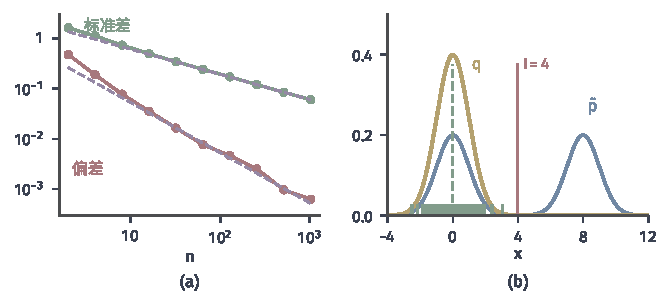
\includegraphics[width=112mm]{figures/07-probability/08-sampling-and-integration/matplotlib/vr-snis/figure.pdf}
 \caption{自归一化估计的偏差与覆盖问题。(a)目标$\operatorname{Gamma}(3,1)$，$f(x)=x$，建议$\operatorname{Exp}(1/2)$；每个$n$独立重复$4\times10^{4}$次（种子5），绿线为估计的标准差，红线为偏差的绝对值，紫色虚线为渐近参照$\sqrt{3.687/n}$与$0.527/n$。(b)目标$\widetilde{p}=\tfrac12\varphi(x)+\tfrac12\varphi(x-8)$（蓝线），建议$\mathcal{N}(0,1)$（黄线）；绿色短线为前$200$个建议样本，绿色虚线为$n=1000$时的估计值，红线为真值$4$。}
 \label{fig:vr-snis}
\end{BookInlineFigure}

\paragraph{权重的有效样本量看不到漏掉的区域}
实践中常用权重计算
\[
 n_{\mathrm{w}}=\frac{\bigl(\sum_{i=1}^{n}\widetilde{w}_i\bigr)^2}{\sum_{i=1}^{n}\widetilde{w}_i^2} .
\]
它介于$1$与$n$之间：权重全相等时为$n$，一个权重压倒其余时接近$1$。上面的五点例子中$n_{\mathrm{w}}=3.88$。它衡量的是已经抽到的样本之间权重的分散程度，看不到没有抽到的地方。

图~\ref{fig:vr-snis}(b)是一个反例。目标是两个相距$8$的正态峰的等权混合，真值$\mathbb{E}_P[X]=4$；建议$\mathcal{N}(0,1)$只盖住左峰。覆盖条件成立（$q$处处为正），所以定理~\ref{thm:vr-sn-consistency}保证估计最终收敛到$4$。但权重
\[
 \widetilde{w}(x)=\tfrac12+\tfrac12\mathrm{e}^{8x-32}
\]
只在$x>4$附近才明显偏离$\tfrac12$，而建议样本进入那里的概率约为$3\times10^{-5}$。$n=1000$（种子6）时，估计值为$-0.012$，而$n_{\mathrm{w}}=1000.0$：所有权重几乎相同，指标显示“完美”，估计却错了整整一个峰。经验指标稳定不能证明建议分布覆盖了目标的重要区域。
